\documentclass[12pt,a4paper]{article}
\usepackage[utf8]{inputenc}
\usepackage[spanish,es-tabla,es-noquoting]{babel}
\usepackage{geometry}
\usepackage{graphicx}
\usepackage{multirow}
\usepackage{tabularx}
\usepackage{longtable}
\usepackage{float}
\usepackage{amsmath}
\usepackage{amssymb}
\usepackage{mathptmx}
\usepackage{fancyhdr}
\usepackage{array}
\usepackage[table]{xcolor}
\usepackage{titlesec}
\usepackage{setspace}
\usepackage{microtype}
\usepackage{lastpage}
\usepackage{booktabs}
\usepackage{enumitem}
\usepackage{hyperref}
\usepackage{listings}

\hypersetup{
    colorlinks=true,
    linkcolor=black,
    citecolor=blue!70!black,
    urlcolor=blue!70!black
}

\graphicspath{{images/}{../images/}{./}}

\geometry{
    top=4.7cm,
    bottom=2.5cm,
    left=2.5cm,
    right=2.5cm,
    headheight=3.9cm,
    headsep=0.4cm
}

\setstretch{1.15}
\setlength{\parindent}{0pt}
\setlength{\parskip}{0.45em}
\setlength{\tabcolsep}{4pt}

\titleformat{\section}
  {\normalfont\fontsize{12}{14.5}\bfseries}{\thesection.}{0.6em}{\uppercase}
\titlespacing*{\section}
  {0pt}{1.8ex plus 0.4ex minus 0.2ex}{0.6ex plus 0.2ex}

\titleformat{\subsection}
  {\normalfont\fontsize{11.5}{13.5}\bfseries}{\thesubsection.}{0.5em}{}
\titlespacing*{\subsection}
  {0pt}{1.4ex plus 0.3ex minus 0.1ex}{0.4ex plus 0.1ex}

\titleformat{\subsubsection}
  {\normalfont\fontsize{10.5}{12.5}\bfseries\itshape}{\thesubsubsection.}{0.4em}{}
\titlespacing*{\subsubsection}
  {0pt}{1.1ex plus 0.2ex minus 0.1ex}{0.3ex plus 0.1ex}

\newcolumntype{Y}{>{\centering\arraybackslash}X}
\newcolumntype{L}{>{\raggedright\arraybackslash}X}
\newcolumntype{C}{>{\centering\arraybackslash}X}

\definecolor{headerred}{RGB}{180, 0, 0}
\definecolor{darkred}{RGB}{140, 0, 0}
\definecolor{lightgraybg}{RGB}{248, 248, 248}
\definecolor{tableheader}{RGB}{232, 238, 246}
\definecolor{navyheader}{RGB}{0, 52, 94}

\newcommand{\docCodigo}{TI-SIGE-ENT-F3-013}
\newcommand{\docVersion}{1.0}
\newcommand{\docProceso}{INGENIERÍA DE SOFTWARE / ASISTENCIA CON INTELIGENCIA ARTIFICIAL}
\newcommand{\docElaboracion}{07/10/2026}
\newcommand{\docRevision}{07/10/2026}
\newcommand{\docTitulo}{INTEGRACIÓN DE LA CAPA DE IA: GOOGLE GEMINI API Y MOTOR HEURÍSTICO}
\newcommand{\docOrganizacion}{FACULTAD DE INGENIERÍA EN SISTEMAS, ELECTRÓNICA E INDUSTRIAL}
\newcommand{\docSubOrganizacion}{CARRERA DE INGENIERÍA DE SOFTWARE}

\newcommand{\encabezadofrecuente}{%
    \renewcommand{\arraystretch}{1.15}%
    \noindent\makebox[\textwidth][c]{%
    \begin{tabularx}{\textwidth}{|>{\centering\arraybackslash}m{2.8cm}|Y|>{\centering\arraybackslash}m{4.8cm}|}
        \hline
        \multirow{4}{2.8cm}{\centering\raisebox{-1.15cm}{
\includegraphics[width=2.5cm,height=2.0cm,keepaspectratio]{images/logo.png}}}
        & \textbf{\fontsize{9}{11}\selectfont \docOrganizacion} 
        & \textbf{\fontsize{8}{10}\selectfont CÓDIGO:} \fontsize{8}{10}\selectfont \docCodigo \\
        \cline{3-3}
        & \textbf{\fontsize{8.5}{10.5}\selectfont \docSubOrganizacion} 
        & \textbf{\fontsize{8}{10}\selectfont VERSIÓN:} \fontsize{8}{10}\selectfont \docVersion \\
        \cline{2-3}
        & \textbf{\fontsize{8}{10}\selectfont PROCESO:} \fontsize{8}{10}\selectfont \docProceso 
        & \textbf{\fontsize{8}{10}\selectfont ELABORACIÓN:} \fontsize{8}{10}\selectfont \docElaboracion \\
        \cline{2-3}
        & \textbf{\fontsize{8.5}{10.5}\selectfont \docTitulo} 
        & \textbf{\fontsize{8}{10}\selectfont ÚLTIMA REVISIÓN:} \fontsize{8}{10}\selectfont \docRevision \\
        \hline
    \end{tabularx}%
    }%
}

\pagestyle{fancy}
\fancyhf{}
\fancyhead[C]{\encabezadofrecuente}
\fancyfoot[C]{\fontsize{10}{12}\selectfont Página \thepage\ de \pageref{LastPage}}
\renewcommand{\headrulewidth}{0pt}

\lstset{
  basicstyle=\ttfamily\scriptsize,
  backgroundcolor=\color{lightgraybg},
  frame=single,
  breaklines=true,
  tabsize=2,
  showstringspaces=false
}

\begin{document}

\noindent{\fontsize{10.5}{12.5}\selectfont \textbf{Integrantes:} Heidi Villavicencio \quad$\vert$\quad Steeven Toala \quad$\vert$\quad Nixon Hurtado \quad$\vert$\quad Andrea Vásquez}

\vspace{0.25cm}

\section{Título}
\textbf{Denominación del Entregable:} Integración de la Capa de Inteligencia Artificial: Asistente con Google Gemini 1.5 Flash API y Motor de Respaldo Heurístico Institucional -- Código EDT: 3.13 (Fase 3: Desarrollo Iterativo Core).

\section{Introducción}
La elaboración de los Planes de Trabajo Docente (formato \texttt{UTA-SGC-A-2-1-P7-T1}) y de los Informes Semestrales de Cumplimiento (\texttt{UTA-SGC-A-2-1-P7-T2}) en la FISEI exige coherencia pedagógica entre las asignaturas asignadas, la justificación institucional y los objetivos de aprendizaje formulados de acuerdo con la Taxonomía de Bloom. En el proceso tradicional, los docentes presentaban con frecuencia discordancias sintácticas y demoras al redactar justificaciones y metas semestrales.

Para solucionar este desafío, se diseñó e implementó en la solución SIGE un servicio de asistencia inteligente centrado en la **API de Google Gemini 1.5 Flash** (a través de \texttt{geminiService.js}). Para mitigar caídas de conectividad o limitaciones temporales de cuota, el servicio incorpora un **Motor de Respaldo Heurístico Institucional UTA** y un **Motor de Diff de Versiones**, garantizando asistencia permanente, alta disponibilidad y soporte en auditorías del Sistema de Gestión de Calidad (SGC).

\section{Objetivo}

\subsection{Objetivo General}
Implementar y verificar el servicio de inteligencia artificial basado en la API de Google Gemini 1.5 Flash integrado en la plataforma SIGE, dotándolo de un motor heurístico de contingencia para la asistencia interactiva en la redacción de objetivos, justificaciones y evaluación de coherencia académica.

\subsection{Objetivos Específicos}
\begin{itemize}[leftmargin=1.5em, itemsep=1.5pt]
    \item Integrar el cliente de la API de Google Gemini 1.5 Flash con gestión segura de API Keys mediante almacenamiento local y variables de entorno.
    \item Desarrollar el motor de respaldo heurístico con timeout de 6.5 segundos para proveer recomendaciones institucionales sin interrupciones operativas.
    \item Diseñar las funciones de análisis de coherencia curricular y detección de diferencias (Diff) entre versiones de borradores docentes.
\end{itemize}

\section{Alcance}

\subsection{Límites de Implementación (In-Scope)}
\begin{itemize}[leftmargin=1.5em, itemsep=1.5pt]
    \item Sugerencia de objetivos específicos con verbos de Bloom según el nombre de la materia y área del conocimiento.
    \item Evaluación de coherencia cualitativa entre la justificación redactada y las horas declaradas en la matriz.
    \item Componente de comparación visual de versiones (\texttt{VersionHistoryModal.jsx}) con resaltado de modificaciones.
\end{itemize}

\subsection{Exclusiones (Out-of-Scope)}
\begin{itemize}[leftmargin=1.5em, itemsep=1.5pt]
    \item Aprobación automatizada de planes (la IA es estrictamente un asistente de soporte; la decisión y firma es humana).
    \item Inferencia de modelos no supervisados en servidores locales de alto costo de cómputo.
\end{itemize}

\section{Definiciones}
\begin{itemize}[leftmargin=1.5em, itemsep=2pt]
    \item \textbf{Google Gemini 1.5 Flash API:} Modelo multimodal de lenguaje de alta velocidad y baja latencia desarrollado por Google, optimizado para razonamiento lingüístico en español.
    \item \textbf{Motor de Respaldo Heurístico:} Algoritmo determinístico basado en catálogos de verbos de Bloom y plantillas SGC de la UTA que genera recomendaciones válidas si la API externa no responde en 6.5 segundos.
    \item \textbf{Diff Semántico:} Algoritmo de comparación textual que detecta inserciones, supresiones y alteraciones entre dos versiones sucesivas de un expediente.
    \item \textbf{Human-in-the-Loop:} Principio de diseño donde el usuario docente inspecciona, edita y convalida voluntariamente cualquier sugerencia generada antes de incorporarla al borrador oficial.
\end{itemize}

\section{Responsabilidades}
\begin{itemize}[leftmargin=1.5em, itemsep=2pt]
    \item \textbf{Analista de Requisitos / UI-UX (Heidi Villavicencio):} Relevamiento de necesidades docentes, diseño de la interfaz del asistente modal y pruebas de usabilidad.
    \item \textbf{Líder de Proyecto / Arquitecto de Software (Steeven Toala):} Arquitectura de \texttt{geminiService.js}, diseño del fallback heurístico y control de latencia.
    \item \textbf{Desarrollador Backend / DBA (Nixon Hurtado):} Respaldo en endpoints de persistencia de borradores y almacenamiento de historial de versiones.
    \item \textbf{Desarrolladora Frontend / QA (Andrea Vásquez):} Integración del hook en React, control de estados de carga (\textit{loading/error}) y pruebas de retest.
    \item \textbf{Docente Evaluador / Tutor (Ing. Paulo Torres, Mg.):} Asesoría pedagógica en verbos de Bloom, validación ética y aprobación formal del módulo.
\end{itemize}

\section{Normativa Legal y Técnica}
\begin{itemize}[leftmargin=1.5em, itemsep=2pt]
    \item \textbf{ISO/IEC 25010:2023:} Calidad del software (Usabilidad, Fiabilidad y Tolerancia a Fallos ante caídas de red externa).
    \item \textbf{Ley Orgánica de Protección de Datos Personales (Ecuador):} Restricción de envío de datos de identificación personal en los prompts de inferencia.
    \item \textbf{Políticas de Inteligencia Artificial en Educación Superior (UNESCO):} Principio de transparencia, explicabilidad y autoría responsable del contenido docente.
\end{itemize}

\section{Método, Políticas y Contenidos}
La arquitectura de integración opera bajo las siguientes políticas:
\begin{enumerate}[leftmargin=1.5em, itemsep=2pt]
    \item \textbf{Gestión Descentralizada de Credenciales:} La API Key de Gemini puede suministrarse globalmente mediante variable de entorno (\texttt{VITE\_GEMINI\_API\_KEY}) o por cada docente en su navegador mediante \texttt{localStorage}, evitando la exposición de claves maestras.
    \item \textbf{Tolerancia a Fallos mediante Fallback Automático:} Si la petición a Google Gemini supera el umbral de 6.5 segundos o retorna error 429/500, el sistema activa de forma transparente el motor heurístico UTA sin interrumpir el flujo del docente.
    \item \textbf{Control de Temperatura Reducida ($\mathbf{T = 0.3}$):} La API se parametriza con baja variabilidad para evitar alucinaciones y asegurar terminología académica rigurosa.
\end{enumerate}

\begin{figure}[htbp]
    \centering
    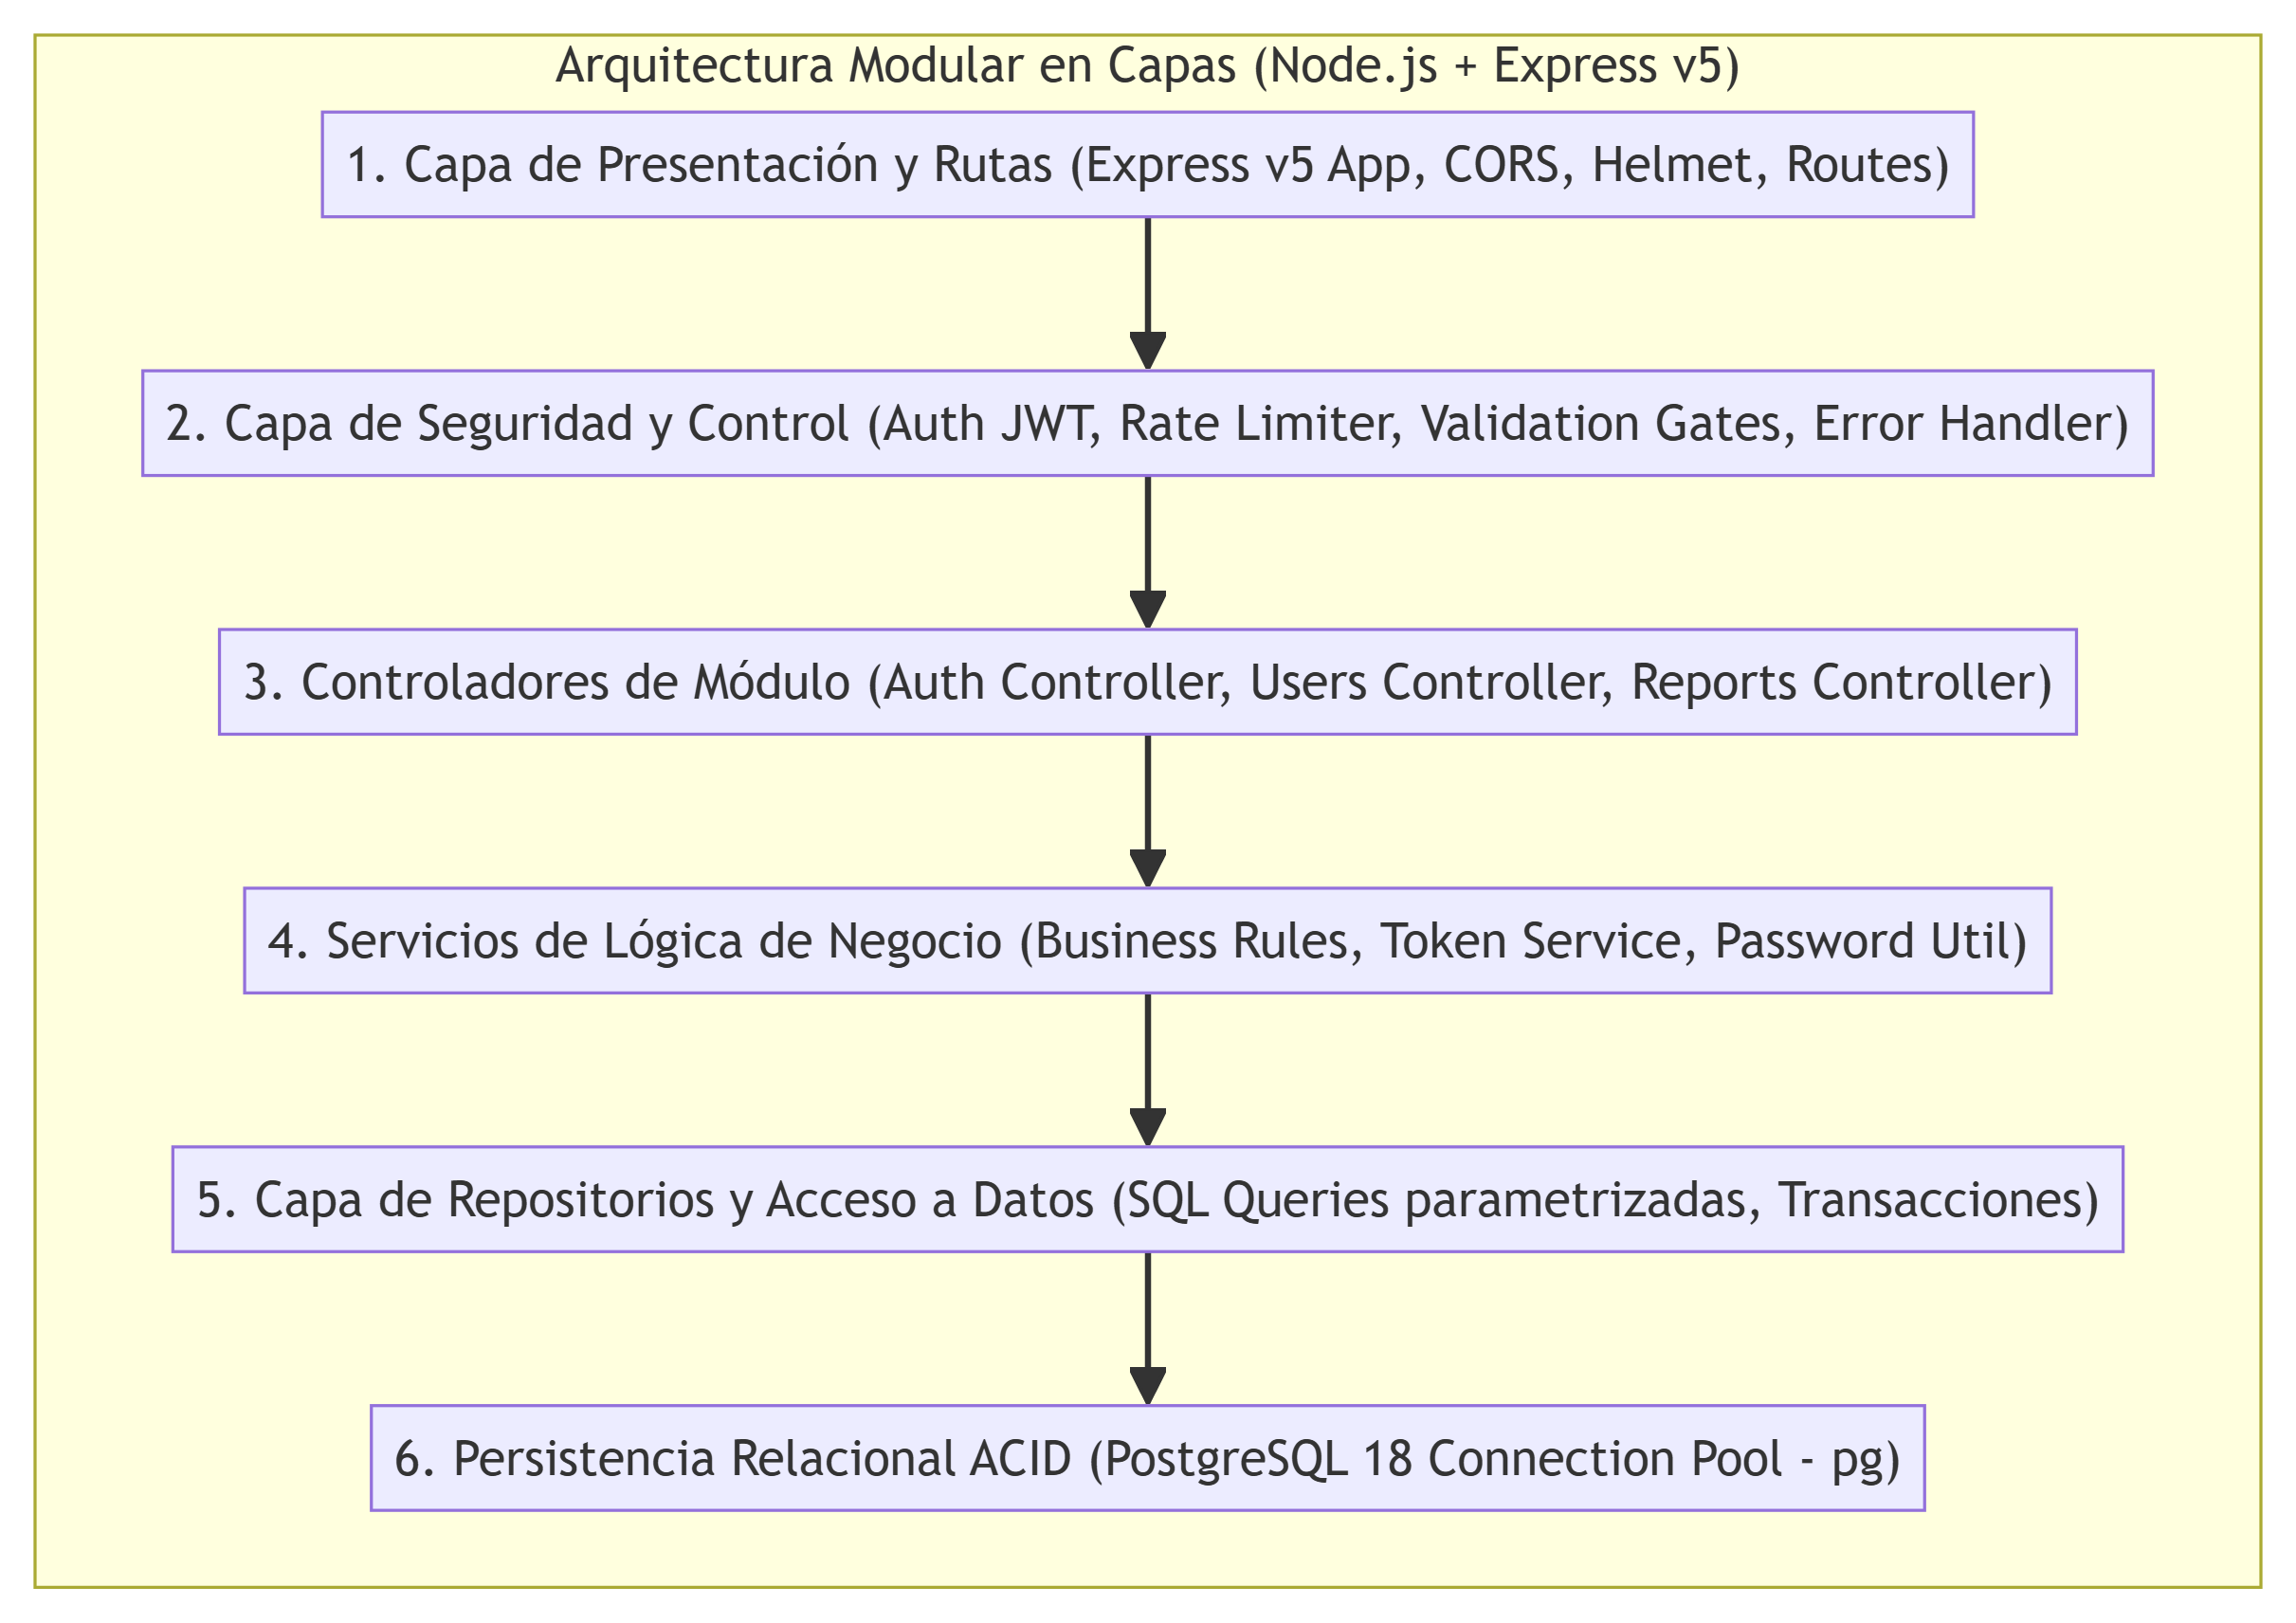
\includegraphics[width=0.88\textwidth,keepaspectratio]{images/s2_02_clean_architecture.png}
    \caption{Arquitectura en Capas de SIGE integrando el Servicio Gemini y Fallback Heurístico.}
    \label{fig:arquitectura_gemini}
\end{figure}

\section{Descripción de actividades}

\subsection{Implementación del Servicio de IA (geminiService.js)}
A continuación se ilustra la arquitectura de invocación y fallback implementada en el cliente frontend:
\begin{lstlisting}[language=JavaScript]
// SIGE/frontend/src/services/geminiService.js
export const callGeminiApi = async ({ prompt, systemInstruction = '', temperature = 0.3 }) => {
  const apiKey = getGeminiApiKey();
  if (!apiKey) throw new Error('NO_API_KEY');

  const url = `https://generativelanguage.googleapis.com/v1beta/models/gemini-1.5-flash:generateContent?key=${apiKey}`;
  
  const payload = {
    contents: [{ role: 'user', parts: [{ text: prompt }] }],
    generationConfig: { temperature, maxOutputTokens: 1024 }
  };

  const response = await fetch(url, {
    method: 'POST',
    headers: { 'Content-Type': 'application/json' },
    body: JSON.stringify(payload)
  });

  const data = await response.json();
  return data.candidates?.[0]?.content?.parts?.[0]?.text || '';
};
\end{lstlisting}

\subsection{Mecanismo de Respaldo Heurístico Institucional}
Si la llamada remota falla, se dispara el motor heurístico local:
\begin{lstlisting}[language=JavaScript]
export const generatePlanDraftAssistance = async ({ materia, carrera, horas = 160 }) => {
  try {
    const prompt = `Actúa como especialista curricular de la FISEI UTA. Materia: ${materia}, Carrera: ${carrera}.
Genera: 1) Justificación institucional SGC, 2) Tres objetivos según Taxonomía de Bloom.`;
    const response = await Promise.race([
      callGeminiApi({ prompt }),
      new Promise((_, reject) => setTimeout(() => reject(new Error('TIMEOUT')), 6500))
    ]);
    return { success: true, source: 'gemini_api', data: response };
  } catch (err) {
    // Activación automática de Fallback Heurístico UTA
    return { success: true, source: 'heuristic_fallback_uta', data: getHeuristicSuggestions(materia) };
  }
};
\end{lstlisting}

\begin{figure}[htbp]
    \centering
    
\includegraphics[width=0.88\textwidth,keepaspectratio]{images/plan_page_2.png}
    \caption{Asistente de IA Integrado en la Vista de Justificación y Objetivos de SIGE.}
    \label{fig:gemini_ui_preview}
\end{figure}

\section{Firmas de Responsabilidad}

\noindent
\renewcommand{\arraystretch}{1.2}
\begin{tabularx}{\textwidth}{|>{\raggedright\arraybackslash}m{2.9cm}|>{\raggedright\arraybackslash}X|>{\centering\arraybackslash}m{4.6cm}|>{\centering\arraybackslash}m{2.3cm}|}
    \hline
    \rowcolor{tableheader}
    \textbf{ACCIÓN} & \textbf{NOMBRE Y CARGO} & \textbf{FIRMA} & \textbf{FECHA} \\
    \hline
    \textbf{Elaborado por:} & Heidi Villavicencio\newline Analista de Requisitos / UI-UX & \parbox[c]{4.4cm}{\centering\vspace{4pt}
\includegraphics[height=1.5cm,width=4.0cm,keepaspectratio]{images/firma_heidi.png}\vspace{4pt}} & 07/10/2026 \\
    \hline
    \textbf{Revisado por:} & Steeven Toala\newline Líder de Proyecto / Arquitecto & \parbox[c]{4.4cm}{\centering\vspace{4pt}
\includegraphics[height=1.5cm,width=4.0cm,keepaspectratio]{images/firma_steveen.png}\vspace{4pt}} & 07/10/2026 \\
    \hline
    \textbf{Aprobado por:} & Ing. Paulo Torres, Mg.\newline Docente Evaluador -- Gestión Proyectos & \parbox[c]{4.4cm}{\centering\vspace{8pt}\textbf{\textcolor{gray!80}{\scriptsize [ PENDIENTE DE APROBACIÓN ]}}\vspace{8pt}} & \textbf{\textcolor{gray!90}{Pendiente}} \\
    \hline
\end{tabularx}

\vspace{0.4cm}

\section{Control de Cambios}

\noindent
\renewcommand{\arraystretch}{1.2}
\begin{tabularx}{\textwidth}{|>{\hsize=0.45\hsize\centering\arraybackslash}X|>{\hsize=1.55\hsize\raggedright\arraybackslash}X|>{\hsize=1.2\hsize\raggedright\arraybackslash}X|>{\hsize=0.8\hsize\centering\arraybackslash}X|}
    \hline
    \rowcolor{tableheader}
    \textbf{Versión} & \textbf{Descripción del cambio} & \textbf{Responsable del cambio} & \textbf{Fecha de aprobación} \\
    \hline
    1.0 & Integración de Google Gemini 1.5 Flash API con fallback heurístico institucional y motor de diff de versiones en frontend. & Steeven Toala / Heidi Villavicencio & 07/10/2026 \\
    \hline
\end{tabularx}

\vspace{0.4cm}

\section{Anexos}

\subsection*{Anexo 1: Catálogo de Verbos de la Taxonomía de Bloom Integrados en el Motor Heurístico}
\begin{table}[H]
\centering
\small
\begin{tabularx}{\textwidth}{|l|X|}
\hline
\rowcolor{tableheader}
\textbf{Nivel Cognitivo de Bloom} & \textbf{Verbos de Acción Validados en el Motor Institucional} \\ \hline
1. Recordar / Conocer & Definir, describir, identificar, listar, nombrar, reconocer, reproducir. \\ \hline
2. Comprender & Clasificar, explicar, interpretar, resumir, traducir, ejemplificar. \\ \hline
3. Aplicar & Implementar, calcular, ejecutar, construir, emplear, utilizar, demostrar. \\ \hline
4. Analizar & Diferenciar, descomponer, organizar, examinar, estructurar, contrastar. \\ \hline
5. Evaluar & Validar, juzgar, auditar, verificar, justificar, evaluar, defender. \\ \hline
6. Crear / Diseñar & Diseñar, formular, proponer, construir, modelar, desarrollar, planificar. \\ \hline
\end{tabularx}
\caption{Verbos de Bloom Estructurados para Recomendación de Objetivos en SIGE.}
\label{tab:anexo_bloom}
\end{table}

\end{document}
